\chapter{Background}
\index{Background%
@\emph{Background}}%

When the Web was first created by Tim Berners-Lee in 1989, web pages were largely envisioned as static \textit{documents} with a single author or a small group of coordinating authors. 
The idea of composing a complex web application out of simple components like snapping together Lego blocks seemed like a distant dream at best.
Until recently, web authors were limited to using the predefined HTML elements or `tags` that were listed in the W3C standard and understood by browser programs, such as \tcode{<title>} and \tcode{<video>}. 
Creating your own \textit{sui generis} HTML elements with unique behaviors seemed beyond the capabilities of the web browsers of the day like Mosaic and Netscape Navigator.

As of early 2015, `modern' web apps are typically written with a Javascript framework that provides a cohesive set of structures, design patterns and practices designed to facility composing web applications, large or small, from a number of sub-components.
The difference between a `framework` and a library is somewhat arbitrary but typically frameworks are more comprehensive than narrowly focused utility libraries.
Yet all frameworks must exist within the confines of the programming model provided by the browser and the Document Object Model (DOM). 
In this model, the entire web page or app belongs to a single `document', constituent parts are not encapsulated or isolated from each other, and authors are limited to working with the predefined HTML tags.
These issues make it difficult to create and share generic, reusable \textit{web components} 
--- in the abstract sense --- 
among different users who may not follow the same set of assumptions or conventions.

\section{Current challenges in web authoring}
To illustrate how these problems affect the ability of authors to share and reuse code, let's look at an example from the popular Twitter Bootstrap library [CITE].
Twitter Bootstrap is a collection of Cascading Style Sheet (CSS) rules and Javascript widgets or components designed to allow web authors to quickly ``bootstrap'' an attractive, consistent look-and-feel onto a web page.
Bootstrap provides styled User Interface (UI) widgets such as menus, buttons, panels, `dropdown' selectors, alerts, dialogs, and so on, to be used as building blocks to construct web sites or applications.
Because Bootstrap must work within the confines of the DOM and the HTML5 standard, this necessarily exposes a great deal of Bootstrap's internals to authors that wish to use it. 
For example, to add a Bootstrap site navigation bar to your page, you must copy and paste a large block of HTML and then customize it to your needs as shown in figure~\ref{f:twbs1}.

% 
\begin{figure}[htb]
\centering
 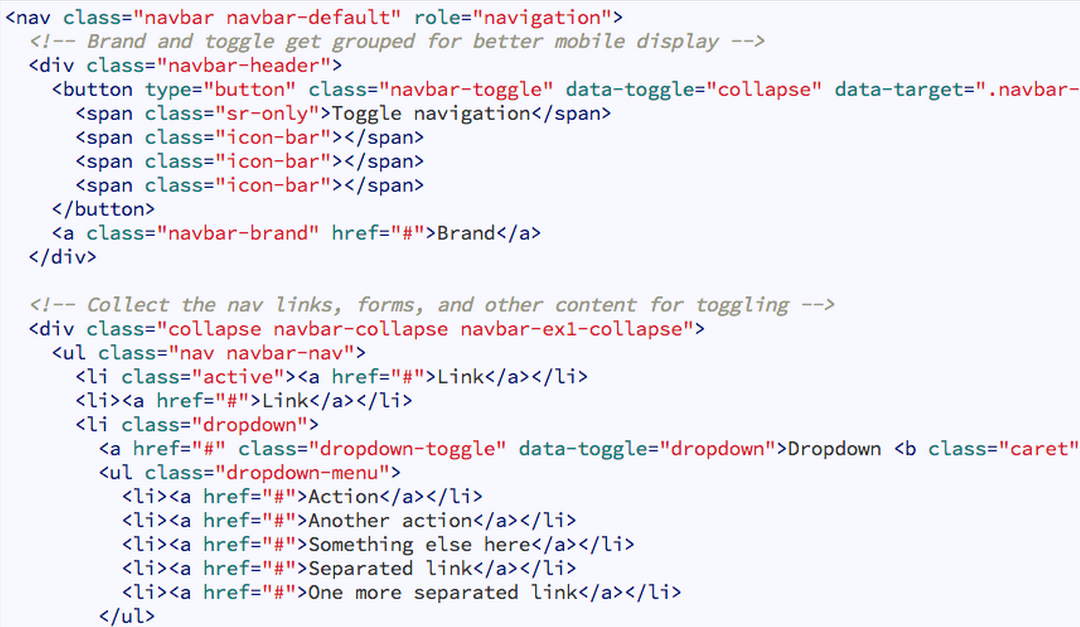
\includegraphics[width=6in]{images/bootstrap_navbar_html.png}
\caption{A partial example of Twitter Bootstrap navigation bar HTML.}
\label{f:twbs1}
\end{figure}
\index{commands!environments!figure}%

This forces users of the library to tightly couple the layout of their page with the internal structure required by Bootstrap's navigation bar widget. 
This coupling militates against Bootstrap refactoring or modifying the internal structure of the navigation widget because this would require the large community of users to update their applications accordingly.
In addition, because CSS rules normally apply across the entire page, the authors of Bootstrap must carefully select the scope and nomenclature of all rules to ensure minimal interference with other components and unintended effects. 
Even then, conflicts are inevitable when the entire page is treated as a single sandbox. 
In short, there is no encapsulation between components. 
In fact, neither HTML5 nor Javascript (ECMAScript 5) have a well-defined notion of a discrete `component' [CITE].

What if instead one could create and share a reusable chunk of functionality --- a web component -- that hid all of these tedious structural details and encapsulated its private, internal state? 
What if web authors could create their \textit{own} HTML elements?  
Using Bootstrap's navigation bar could be as simple as replacing the code in figure~\ref{f:twbs1} with a custom element like the one in figure~\ref{f:twbs2}.

% 
\begin{figure}[htb]
\centering
 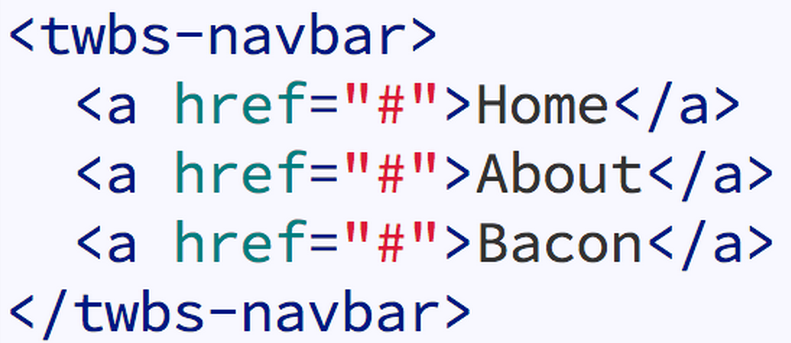
\includegraphics[width=3.5in]{images/bootstrap_navbar_wc.png}
\caption{Hypothetical Bootstrap nav bar custom element.}
\label{f:twbs2}
\end{figure}
\index{commands!environments!figure}%


\subsection{Encapsulation and composition}

The Web Components working group, consisting of software engineers from several major browser vendors, looked at this situation and found that, in practice, browsers already had a suitable model for encapsulating components that hide complexity behind well-defined interfaces.
That model was that one used internally by browsers to implement the newer HTML5 tags like the \textbf{\tcode{<video>}} element. 
The \tcode{<video>} element presents a simple interface (API) to HTML authors that hides the complexities of playing high definition video.
Internally, however, browsers implement \tcode{<video>} with a `shadow' hidden document inside the object that contains the internal state. 
For example, an author can write \texttt{<video loop src=...>} to cause the video to loop repeatedly.

This shadow Document Object Model (DOM) inside the \tcode{<video>} tag creates the user interface (UI) needed to control video playback such as volume controls, a timeline bar and pause and play buttons.
These inner playback controls are themselves built out of HTML, CSS and JS but these details are not exposed to web authors who simply place a \tcode{<video>} element on their page. 
Figure~\ref{f:html5video} illustrates how this works. It shows the shadow (internal) DOM of a \tcode{<video>} element on a page with the \tcode{<div>} for the Play button highlighted.

% 
\begin{figure}[htb]
\centering
 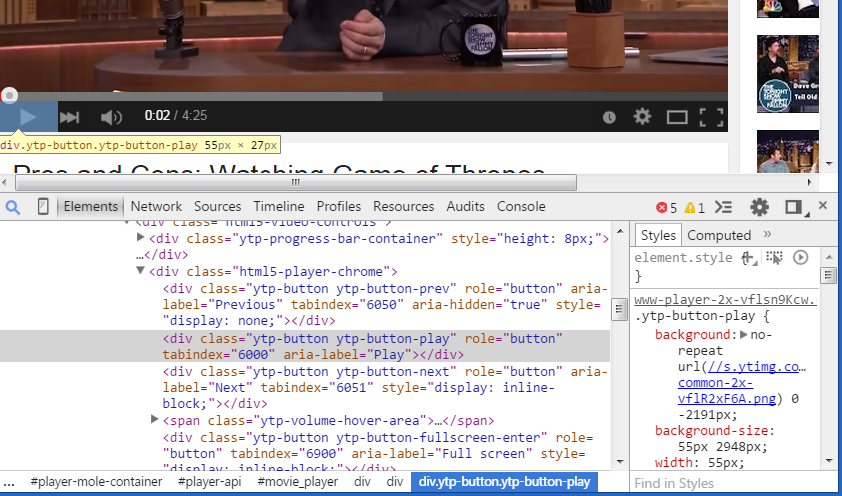
\includegraphics[width=5.5in]{images/html5_video_control.png}
\caption{Opera's \textit{shadow DOM} for \tcode{<video>} and its Play button}
\label{f:html5video}
\end{figure}
\index{commands!environments!figure}%

This design illustrates two principles that are widely followed in other areas of software engineering:

\begin{itemize}
\item Use \textbf{encapsulation} and well defined interfaces as the \tcode{<video>} element does to protect private state and hide implementation complexity.
\item Prefer \textbf{composition} or \textit{has-a} relationships over inheritance or \textit{is-a} relationships when building modules. 
In the case of \tcode{<video>}, it's composed of simple block elements and scoped CSS roles and the Volume and Play controls aren't ``special'' objects, just \texttt{<divs>} with CSS rules and click handlers.
\end{itemize}

The solution, therefore, to these coupling problems in web authoring was expose these internal brower APIs for creating elements in a safe and portable fashion. 
This would allow web authors to create their own rich custom elements using standard portable APIs, encapsulate their internals, and share them with others.
The question remained, which specific browser features needed to be standardized in order to support Web Components?

\section{Web Components}

The Web Component initiate consists of two main technologies and two supporting features. The main technologies are Custom HTML Elements and the Shadow DOM, while HTML Imports and Templates support these features.

\subsection{Custom HTML elements}
Never before have web authors been able to define their own custom HTML elements not found in the official list.
Actually, many authors and web frameworks have done exactly that for years, primarily for internal pre-processing purposes.
The custom elements would not get sent to the end-user's browser because the browser would not understand what to do with them.
However the possibility now exists to create custom elements in a standard way that will be supported by browsers.
The primary restriction to avoid a name collision with future built-in HTML elements is that all custom elements must have a \texttt{-} character (dash) in their name, such as \texttt{<my-element>}.

\subsection{Shadow DOM}
Shadow DOM is available to any element, not just custom elements, but the primary need for them is to encapsulate the internals of custom elements.
\subsection{HTML Imports}
\subsection{Templates}
\subsection{Related technologies}

\section{Literature Review}
\subsection{Popular Javascript frameworks}
\subsection{Google Polymer framework}

\section{Speakur}
\subsection{Origin}
\subsection{Motivations}

